\section{Lecture 13: Causality of LSI systems}




\subsection{Associativity and Commutativity of LSI Systems}
Two more properties of system, namely associativity and commutativity are explored here. These properties are not "new" in the sense that some basic operations like addition and multiplication follow these properties.
Note: Both discrete and continuous systems are considered together in the following discussion.

\subsubsection{Associativity}
\begin{figure}[ht]
\centering
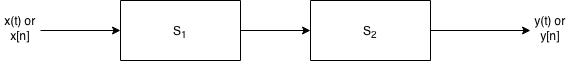
\includegraphics[width=0.8\textwidth]{cascade1.jpg}
\end{figure}

In the above image, we input signal $x$, either $x(t)$ for continuous system or $x[n]$ for discrete one, to LSI system $S_{1}$( having its impulse response $h_{1}(t)$ or $h_{1}[n]$), which can be considered continuous or discrete, depending on the case. The output of system $S_{1}$ is fed to LSI system $S_{2}$( having its impulse response $h_{2}(t)$ or $h_{2}[n]$), which also can be continuous or discrete. The output of $S_{2}$ is $y$, either $y(t)$ or $y[n]$ in continuous and discrete case respectively. That is, the whole setup can be considered either of the continuous or the discrete case. In the continuous case, both the systems as well as the relevant signals are continuous, whereas in discrete case they all operate on a discrete independent variable.\\
Note here, that the output obtained from the first system is $(x*h_{1})$, continuous or discrete. As this signal is fed to the $S_{2}$, we get output as 
\begin{equation}
y=(x*h_{1})*h_{2} \nonumber
\end{equation}

Now Associativity talks about the equivalence of systems put in series or cascade. Mathematically,
\begin{equation}
(x*h_{1})*h_{2}=x*(h_{1}*h_{2}) \nonumber
\end{equation}

Now if we have a LSI system $S_{3}$, whose impulse response is $h_{1}*h_{2}$, then from above equation it is clear that it will act exactly like these two systems $S_{1}$ and $S_{2}$ would have acted when applied in series. This is the physical significance of the associativity.\\

\begin{figure}[ht]
\centering
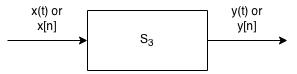
\includegraphics[width=0.5\textwidth]{eqv.jpg}
\end{figure}

So  in short, if we put two systems in a cascade, we can replace them with one single system whose impulse response is equal to the convolution of the impulse responses of these two systems.

\subsubsection{Commutativity}

Let us apply signal $x$ to system $S_{1}$ and then its output to system $S_{2}$, both LSI, to get output as $y$. Commutativity states that the order in which these systems come is irrelevant to the result i.e. we will get the same output in both the cases.  It states that regardless of which of the two systems comes first, the output $y$ is going to be the same.\\

\begin{figure}[ht]
\centering
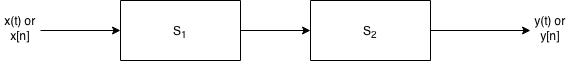
\includegraphics[width=0.8\textwidth]{cascade1.jpg}
\end{figure}
\begin{figure}[ht]
\centering
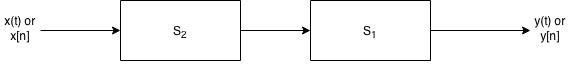
\includegraphics[width=0.8\textwidth]{cascade2.jpg}
\end{figure}

So the equivalent system which we talked about in the Associativity, is unaffected if the order of these two systems is reversed.\\\\

We can also generalize this to n cascaded LSI systems and say that for any permutation of the given n systems, the output is going to be the same. The proof of this is a bit more intricate and is left an as exercise to the student. The proof can be done by using the method of mathematical induction.

\subsubsection{What if my systems are not LSI?}

All of the above discussion is based on the assumption that all the systems we are considering are LSI in nature. While it may be tempting to generalize these seemingly simple results to all systems, and many times we tend to forget to confirm that the system in question is LSI or not before applying such properties, we must be careful. \\
It turns out that the commutativity and associativity may not hold if the systems $S_{1}$ and $S_{2}$ are not both LSI. For example,\
Let's say system $S_{1}$ is given by the equation $y(t)=(x(t))^2$ and $S_{2}$ by $y(t)=x(t)+1$. We have taken here continuous variable signals and systems, but the same discussion is valid for the discrete case as well. So if we apply first $S_{1}$ and then $S_{2}$, we will get $y(t)=(x(t))^2 +1$ as the output, while reversing the order, i.e. first applying $S_{2}$ and then $S_{1}$ would yield $y(t)=(x(t)+1)^2$. So the both outputs are clearly different.\\
But this does not mean that we can hurry and conclude that the resultant systems will {\it never} be the same. Consider, say, $S_{1}$ as $y(t)=x(t)+4$ and $S_{2}$ as $y(t)=x(t)-4$. Now in this case, regardless of which system comes first, we get output $y(t)=x(t)$.\\
Basically, if even one of the systems is not LSI, we cannot say anything about whether those systems follow associativity or commutativity beforehand: we must examine those systems carefully and determine the answer for the individual case.


\subsection{Causality of a Linear Shift Invariant System from its Impulse Response}

We have noted before that a LSI system can be represented by its impulse response, i.e. we know everything about a system once we know its impulse response. We have seen system properties like causality and stability: according to the previous statement, we should be able to know whether a system is stable and/or causal just by looking at and examining its impulse response. The conditions turn out to be very similar for continuous and discrete variable systems and their respective impulse responses.

\subsubsection{Causality of continuous variable LSI systems}

We say that a system is causal when its output depends only on the past and the current inputs, and {\it not} on the future inputs. We know that, for a continuous independent variable system $S$` having impulse response $h$t, we can relate its input and output by the equation
\begin{equation}
y(t)=\int_{-\infty}^{+\infty} h(\tau)x(t-\tau)\,d\tau \nonumber
\end{equation}

Note that as $\tau$ goes from ${-\infty}$ to ${+\infty}$, $t-\tau$ also goes from ${-\infty}$ to ${+\infty}$. Note that $\tau$ being positive corresponds to the past ( as $t-\tau < t$ when $\tau$ is positive and '$t$' is the current timeframe) while $\tau$ negative to the future and 0 to the current time. Now for the system being causal, we want to eliminate the future inputs, so we must have $h(\tau)$ 0 when $\tau$ is negative, so that there's no contribution of the future terms to the $y(t)$, the output. Note that $h(\tau)=0$ when $\tau<0$ is sufficient condition for causality of the system. It is easy to prove that this condition is also necessary for the system to be causal i.e. there can be no system which is causal that violates this condition. The proof can be done by using the method of proof by contradiction.

\subsubsection{Causality of discrete variable LSI systems}

For discrete systems, we have the following equation relating output to the input(s):
\begin{equation}
y[n]=\sum_{\kappa=-\infty}^{+\infty} h[\kappa]x[n-\kappa] \nonumber
\end{equation}
Similar to the argument for the continuous case, $\kappa<0$ corresponds to the future, $\kappa>0$ to the past and $\kappa=0$ to the present/current input. So causality will be ensured if all the future inputs are cut off, i.e. $h[\kappa]=0,\, \forall \kappa<0$. This is the sufficient condition for  system to be causal. We can also prove the sufficiency by one more way:\\
Consider signals $x_{1}[n]$ and $x_{2}[n]$ such that $x_{1}[n]=x_{2}[n]\, \forall n \le n_{0}$.\\ Note that $x_{1}[n]$ may not be the same as $x_{2}[n]$ for any $n \geq n_{0}.$ Also, from given condition( we are assuming the condition we arrived at to reach at the conclusion that the system is causal)  $h[\kappa]=0 \forall \kappa<0$\\
Now if the system is causal, we must be able to reach  $y_{1}[n]=y_{2}[n]\, \forall n \le n_{0}$.\\
Consider
\begin{equation}
y_{1}[n]=\sum_{\kappa=0}^{+\infty} h[\kappa]x_{1}[n-\kappa],  n \le n_{0} \nonumber
\end{equation}
Note that we started the sum from 0 as before zero, in$-\infty$ to 0 region, we already know that  $h[\kappa]=0$.
Now observe the summation. it contains $x_{1}[n-\kappa]$. But as $\kappa$ is less than 0, we have $n-\kappa>n$, or  $x_{1}[n-\kappa]= x_{2}[n-\kappa]$.\\
So the sum can be converted to 
\begin{equation}
y_{1}[n]=\sum_{\kappa=0}^{+\infty} h[\kappa]x_{2}[n-\kappa] \nonumber
\end{equation}
And the right hand side of the equation is essentially $y_{2}[n]$.\\
Hence  $y_{1}[n]=y_{2}[n] \forall n \le n_{0}$. Hence the sufficiency of the condition is proved. The necessity can also be proved, by using proof by contradiction.
